%%
%% This is file `sample-acmsmall-submission.tex',
%% generated with the docstrip utiThis report presents comparative analysis of five membership testing algorithms for billion-scale username datasets: linear search, binary search, disk-based hash table with linear probing, Bloom filter~\cite{bloom1970}, and Cuckoo filter~\cite{fan2014}. The LoginChecker system implements these algorithms using memory-mapped storage for efficient handling of large datasets. Experimental validation demonstrates consistent algorithmic performance, with Bloom filters tested up to 1 billion elements due to time constraints, while disk-based hash tables and Cuckoo filters are theoretically capable of similar scaling. Linear search becomes impractical beyond 100K elements. The disk-based implementation choice enables persistent storage and memory-efficient processing, making billion-scale experiments feasible on standard hardware. Complete implementation available~\cite{loginchecker}.ity.
%%
%% The original source files were:
%%
%% samples.dtx  (with optio\textbf{Scale selection:} Experiments used exponential sizing from 100 to 1 billion usernames: [100, 500, 1K, 5K, 10K, 50K, 100K, 500K, 1M, 5M, 10M, 50M, 100M, 500M, 1B]. Algorithm-specific limits were applied based on practical performance constraints and time limitations: linear search ($\leq$100K), binary search ($\leq$100M), Cuckoo filter ($\leq$10M), while Bloom filter was tested up to 1B elements. Disk HashSet and Cuckoo filter are theoretically capable of billion-scale performance but were limited by experiment duration due to setup time requirements.
%% 
%% IMPORTANT NOTICE:
%% 
%% For the copyright see the source file.
%% 
%% Any modified versions of this file must be renamed
%% with new filenames distinct from sample-acmsmall-submission.tex.
%% 
%% For distribution of the original source see the terms
%% for copying and modification in the file samples.dtx.
%% 
%% This generated file may be distributed as long as the
%% original source files, as listed above, are part of the
%% same distribution. (The sources need not necessarily be
%% in the same archive or directory.)
%%
%%
%% Commands for TeXCount
%TC:macro \cite [option:text,text]
%TC:macro \citep [option:text,text]
%TC:macro \citet [option:text,text]
%TC:envir table 0 1
%TC:envir table* 0 1
%TC:envir tabular [ignore] word
%TC:envir displaymath 0 word
%TC:envir math 0 word
%TC:envir comment 0 0
%%
%% The first command in your LaTeX source must be the \documentclass
%% command.
%%
%% For submission and review of your manuscript please change the
%% command to \documentclass[manuscript, screen, review]{acmart}.
%%
%% When submitting camera ready or to TAPS, please change the command
%% to \documentclass[sigconf]{acmart} or whichever template is required
%% for your publication.
%%
%%
 \documentclass[sigconf]{acmart} 
 \settopmatter{printacmref=false} % removes ACM reference format
\renewcommand\footnotetextcopyrightpermission[1]{} % removes "permission" block
\pagestyle{plain} % removes headers
%%
%% \BibTeX command to typeset BibTeX logo in the docs
\AtBeginDocument{%
  \providecommand\BibTeX{{%
    Bib\TeX}}}
\setcopyright{none}
\usepackage{url}

%%
%% end of the preamble, start of the body of the document source.
\begin{document}

%%
%% The "title" command has an optional parameter,
%% allowing the author to define a "short title" to be used in page headers.
\title{Assignment 1 - LoginChecker}

%%
%% The "author" command and its associated commands are used to define
%% the authors and their affiliations.
%% Of note is the shared affiliation of the first two authors, and the
%% "authornote" and "authornotemark" commands
%% used to denote shared contribution to the research.
\author{Fahd Seddik}
\email{fseddik@student.ubc.ca}
\affiliation{%
  \institution{University of British Columbia}
  \city{Kelowna}
  \state{British Columbia}
  \country{Canada}
}

%%
%% This command processes the author and affiliation and title
%% information and builds the first part of the formatted document.
\maketitle


\section{Introduction}
This report implements and compares five membership testing algorithms for the LoginChecker system, designed to handle billion-scale username datasets. I chose a disk-based implementation approach using memory-mapped files to enable processing of datasets that exceed available RAM. The study provides: (1) parameterized complexity analysis for each algorithm, (2) mathematical justifications for complexity bounds, (3) experimental validation with datasets ranging from 100 usernames to 1 billion usernames, and (4) performance comparison across different scales. The implementation leverages Python with memory-mapped storage, MurmurHash3~\cite{mmh3docs} for hashing, and comprehensive benchmarking infrastructure.

Complete implementation available at: \textcolor{blue}{\url{https://github.com/FahdSeddik/LoginChecker}}~\cite{loginchecker}

\section{Notation and parameters}
I use the following symbols throughout the report:
\begin{itemize}
\item $n$: number of elements stored (or estimated number of elements for probabilistic structures).
\item $m$: number of slots / bits / buckets depending on the structure.
\item $k$: number of independent hash functions (Bloom filter).
\item $f$: fingerprint size in bits (Cuckoo filter).
\item $b$: bucket size (number of entries per bucket in Cuckoo filter).
\item $\alpha$: load factor ($\alpha = n/m$) for hash tables or cuckoo tables.
\item $\varepsilon$: false-positive probability (for Bloom / Cuckoo filters).
\item $h_1, h_2$: two independent hash functions for Kirsch-Mitzenmacher optimization.
\end{itemize}

\section{Complexity analyses and justification}
Each subsection gives (i) a concise statement of time/space complexity using the parameters above, and (ii) a one-paragraph justification.

\subsection{Linear search}
\textbf{Time:} $\Theta(n)$ worst-case and average for an unordered array.\newline
\textbf{Space:} $\Theta(1)$ extra space (in-place).\newline
\textit{Justification:} Linear (sequential) search checks items one-by-one until the item is found or the array ends. In the worst case (not present or last position) the algorithm inspects all $n$ items; expected number of inspections is $\approx n/2$ for a uniformly random target present scenario, hence $\Theta(n)$. The extra space beyond the input is constant (few index variables).

\subsection{Binary search (sorted array)}
\textbf{Time:} $\Theta(\log n)$ for successful or unsuccessful searches.\newline
\textbf{Space:} $\Theta(1)$ extra space for iterative implementation.\newline
\textit{Justification:} Binary search halves the search interval at each step. The recurrence $T(n)=T(n/2)+O(1)$ solves to $T(n)=\Theta(\log n)$ steps.

\subsection{Disk-based hash table (open addressing with linear probing)}
\textbf{Time:} Average-case: $\Theta(1)$ per operation under uniform hashing with reasonable load factors. Worst-case: $\Theta(n)$ if table becomes full.\newline
\textbf{Space:} $\Theta(m \cdot s)$ where $m = 2^p$ slots and $s = 32$ bytes per slot (fixed-size slots with memory mapping).\newline
\textit{Justification:} The disk-based implementation uses open addressing with linear probing in a memory-mapped file. Each 32-byte slot contains: flag (1 byte), key length (1 byte), fingerprint (8 bytes), key data (20 bytes), and padding (2 bytes). This implementation uses MurmurHash3 for primary hashing with a configurable seed for deterministic behavior. The memory-mapped approach enables billion-scale datasets by leveraging virtual memory, allowing the OS to manage paging between RAM and disk efficiently. With proper load factor management, probe distances remain short, maintaining near-constant search times.

\subsection{Bloom filter (probabilistic membership)}
\textbf{Parameters:} $n$ (expected elements), $m$ (bits in bit-array), $k$ (hash functions).\newline
\textbf{Time:} Insert and query both $\Theta(k)$ time using Kirsch-Mitzenmacher optimization.\newline
\textbf{Space:} $m$ bits stored in memory-mapped file, so space is $\Theta(m)$.\newline
\textbf{False-positive probability (approx.):}
\[
\varepsilon \approx \bigl(1 - e^{-kn/m}\bigr)^k.
\]

For a target false-positive probability \(\varepsilon\), optimal parameters are:
\[
m = \left\lceil -\dfrac{n \ln \varepsilon}{(\ln 2)^2} \right\rceil, \qquad
k = \max\left(1, \left\lfloor \dfrac{m}{n}\ln 2 \right\rfloor\right).
\]

\textit{Justification:} The implementation uses MurmurHash3~\cite{mmh3docs} with Kirsch-Mitzenmacher optimization~\cite{kirsch2008}: instead of computing $k$ independent hashes, it computes two hash values $(h_1, h_2)$ and derives $k$ positions as $g_i(x) = (h_1 + i \cdot h_2) \bmod m$. This reduces hash computations from $k$ to 2 while maintaining independence properties. Memory-mapped storage enables efficient handling of large bit arrays (up to gigabytes) with automatic virtual memory management.

\subsection{Cuckoo filter}
\textbf{Parameters:} $n$ (elements), $m$ (number of buckets), $b$ (entries per bucket), $f$ (fingerprint bits), load factor $\alpha=n/(m\cdot b)$.\newline
\textbf{Time:} Expected $\Theta(1)$ for lookup; insert is expected $\Theta(1)$ but may require up to \texttt{max\_kicks} relocations before failing.\newline
\textbf{Space:} Memory-mapped file with $m \cdot b \cdot f$ bits for fingerprints plus header (so $\Theta(m \cdot b \cdot f)$).\newline
\textbf{False-positive probability:} $\varepsilon \leq \frac{2b}{2^f}$ for reasonable load factors.\newline
\textit{Justification:} The implementation uses partial-key cuckoo hashing with two candidate positions: $h_1 = \text{hash}(\text{key})$ and $h_2 = h_1 \oplus \text{hash}(\text{fingerprint})$. Each element is stored as an $f$-bit fingerprint in one of two possible buckets. Lookups check at most $2b$ slots (constant time). Insertions may trigger a bounded cuckoo eviction process with up to \texttt{max\_kicks} relocations. Unlike Bloom filters, cuckoo filters support deletions and provide exact control over false positive rates. Memory mapping enables persistent storage and efficient access patterns.


\section{Experimental plan and validation}
This section describes how the experiments were conducted.

\subsection{Dataset generation and experimental methodology}
I generate realistic usernames using the Mimesis library~\cite{mimesis} with deterministic seeds for reproducibility. The generation process follows Reddit's username standards, limiting usernames to a maximum of 20 characters and allowing only letters, numbers, underscores, and dashes. This ensures realistic data distributions that reflect common username patterns in production systems. The generation process creates usernames with configurable patterns and stores them in an efficient binary format using the \texttt{EfficientUsernameStorage} class, which creates both data files (\texttt{usernames.dat}) and position indices (\texttt{usernames.idx}) for fast random access.

\textbf{Scale selection:} Experiments used exponential sizing from 100 to 1 billion usernames: [100, 500, 1K, 5K, 10K, 50K, 100K, 500K, 1M, 5M, 10M, 50M, 100M, 500M, 1B]. Algorithm-specific limits were applied based on practical performance constraints and time limitations: linear search ($\leq$100K), binary search ($\leq$100M), Cuckoo filter ($\leq$10M), while Bloom filter was tested up to 1B elements. Disk HashSet and Cuckoo filter are theoretically capable of billion-scale performance but were limited by experiment duration due to setup time requirements.

\textbf{Measurement methodology:} Each benchmark measures search time, setup time (structure initialization), and memory usage (RSS memory). To ensure reliable measurements, I perform 5 warmup runs before data collection, then take the average and standard deviation across 10 measurement runs. The disk-based approach enables these large-scale experiments on standard hardware by leveraging memory mapping for efficient virtual memory management. Benchmarking infrastructure was developed with assistance from Generative AI (Claude Sonnet 4).


\subsection{Implementations}
The LoginChecker system provides comprehensive implementations:
\begin{itemize}
\item \textbf{Linear search:} \texttt{LinearSearch} class with performance tracking
\item \textbf{Binary search:} \texttt{BinarySearch} using \texttt{SortedList} structure
\item \textbf{Disk hash table:} \texttt{DiskHashSet} with memory-mapped storage
\item \textbf{Bloom filter:} \texttt{BloomFilter} with Kirsch-Mitzenmacher optimization
\item \textbf{Cuckoo filter:} \texttt{CuckooFilter} with configurable parameters
\end{itemize}
All implementations feature memory-mapped storage for billion-scale datasets, comprehensive unit test suites, and extensive documentation~\cite{loginchecker}.

\subsection{Measurement methodology}
For each structure I measure:
\begin{itemize}
\item Setup time (time to insert the $n$ keys) in seconds
\item Query time per lookup (average over $Q$ lookups) reported in microseconds with the same warmup and measurement protocol.
\item Memory used (resident size or structure-specific memory) reported in MB.
\end{itemize}

\section{Experimental Results}
All experiments were conducted on a system with 12th Gen Intel Core i5-12600K CPU (10 cores, 16 threads, up to 4.9 GHz), 32GB RAM, and 1TB NVMe SSD storage. The implementation uses Python 3.12+ with memory-mapped files for efficient billion-scale dataset handling. Detailed performance measurements are presented in Tables~\ref{tab:linear-results}--\ref{tab:algorithm-comparison}, with comparative analysis shown in Figures~\ref{fig:search-time-scaling}--\ref{fig:bloom-scaling}.

\subsection{Performance measurement results}
\begin{table}[h]
\caption{Linear search performance scaling}
\scriptsize
\begin{tabular}{rrrrr}
\hline
N & Search & Std Dev & Setup & Memory \\
 & ($\mu$s) & ($\mu$s) & (s) & (MB) \\
\hline
100 & 25.0 & 13.0 & 0.0011 & 61.6 \\
500 & 119.0 & 68.0 & 0.000007 & 63.3 \\
1K & 241.0 & 139.0 & 0.000007 & 63.6 \\
5K & 1201.0 & 704.0 & 0.000006 & 63.8 \\
10K & 2459.0 & 1393.0 & 0.000007 & 63.8 \\
50K & 11941.0 & 7016.0 & 0.000007 & 63.9 \\
100K & 18500.0 & 12495.0 & 0.000006 & 64.6 \\
\hline
\end{tabular}
\label{tab:linear-results}
\end{table}

\begin{table}[h]
\caption{Binary search performance scaling}
\scriptsize
\begin{tabular}{rrrrr}
\hline
N & Search & Std Dev & Setup & Memory \\
 & ($\mu$s) & ($\mu$s) & (s) & (MB) \\
\hline
100 & 5.1 & 0.9 & 0.012 & 274 \\
500 & 6.7 & 1.0 & 0.001 & 274 \\
1K & 7.2 & 0.9 & 0.002 & 274 \\
5K & 8.5 & 1.1 & 0.009 & 274 \\
10K & 9.2 & 1.2 & 0.018 & 274 \\
50K & 10.6 & 1.1 & 0.091 & 276 \\
100K & 11.4 & 1.2 & 0.196 & 277 \\
500K & 13.3 & 2.7 & 1.086 & 283 \\
1M & 14.3 & 3.3 & 2.198 & 291 \\
5M & 20.7 & 7.1 & 11.890 & 280 \\
10M & 28.0 & 12.2 & 24.271 & 283 \\
50M & 38.5 & 12.4 & 121.197 & 1067 \\
100M & 42.9 & 12.0 & 241.710 & 2047 \\
\hline
\end{tabular}
\label{tab:binary-results}
\end{table}

\begin{table}[h]
\caption{Disk HashSet performance scaling}
\scriptsize
\begin{tabular}{rrrrr}
\hline
N & Search & Std Dev & Setup & Memory \\
 & ($\mu$s) & ($\mu$s) & (s) & (MB) \\
\hline
100 & 2.7 & 1.3 & 0.001 & 62 \\
500 & 2.3 & 0.9 & 0.001 & 62 \\
1K & 2.2 & 0.4 & 0.002 & 62 \\
5K & 2.4 & 0.6 & 0.007 & 62 \\
10K & 2.4 & 0.8 & 0.015 & 63 \\
50K & 2.3 & 0.7 & 0.071 & 67 \\
100K & 2.5 & 0.3 & 0.139 & 73 \\
500K & 2.3 & 0.5 & 0.694 & 104 \\
1M & 2.6 & 1.7 & 1.377 & 146 \\
5M & 2.8 & 0.5 & 7.098 & 415 \\
10M & 2.6 & 1.1 & 13.670 & 766 \\
50M & 2.7 & 0.4 & 74.786 & 3069 \\
100M & 2.8 & 0.8 & 200.866 & 6075 \\
\hline
\end{tabular}
\label{tab:disk-results}
\end{table}

\begin{table}[h]
\caption{Bloom filter performance scaling (1\% false positive rate)}
\scriptsize
\begin{tabular}{rrrrr}
\hline
N & Search & Std Dev & Setup & Memory \\
 & ($\mu$s) & ($\mu$s) & (s) & (MB) \\
\hline
100 & 3.2 & 0.5 & 0.001 & 62.8 \\
500 & 3.3 & 0.5 & 0.002 & 64.0 \\
1K & 3.4 & 1.0 & 0.004 & 65.3 \\
5K & 3.5 & 0.4 & 0.013 & 66.7 \\
10K & 3.5 & 0.4 & 0.025 & 68.0 \\
50K & 3.6 & 1.0 & 0.120 & 70.2 \\
100K & 3.7 & 1.2 & 0.235 & 72.4 \\
500K & 4.0 & 1.8 & 1.375 & 85.8 \\
1M & 4.1 & 1.2 & 2.747 & 106.7 \\
5M & 4.4 & 1.0 & 15.192 & 296.9 \\
10M & 4.3 & 0.3 & 30.039 & 507.5 \\
50M & 8.3 & 2.4 & 307.629 & 3559.3 \\
100M & 5.0 & 1.6 & 623.796 & 6802.5 \\
500M & 5.2 & 1.5 & 3323.986 & 16753.2 \\
1B & 52.8 & 102.6 & 5637.886 & 20666.5 \\
\hline
\end{tabular}
\label{tab:bloom-results}
\end{table}

\begin{table}[h]
\caption{Cuckoo filter performance scaling}
\scriptsize
\begin{tabular}{rrrrr}
\hline
N & Search & Std Dev & Setup & Memory \\
 & ($\mu$s) & ($\mu$s) & (s) & (MB) \\
\hline
100 & 2.8 & 1.5 & 0.001 & 61 \\
500 & 2.7 & 1.0 & 0.001 & 61 \\
1K & 2.8 & 0.3 & 0.002 & 62 \\
5K & 2.9 & 0.3 & 0.010 & 62 \\
10K & 2.9 & 0.3 & 0.020 & 62 \\
50K & 2.8 & 1.2 & 0.100 & 64 \\
100K & 2.8 & 0.8 & 0.202 & 65 \\
500K & 2.9 & 1.1 & 0.954 & 77 \\
1M & 3.1 & 1.2 & 2.080 & 95 \\
5M & 3.2 & 1.4 & 18.948 & 203 \\
10M & 3.3 & 0.8 & 240.736 & 363 \\
\hline
\end{tabular}
\label{tab:cuckoo-results}
\end{table}

\begin{table}[h]
\caption{Algorithm comparison: search time in $\mu$s (- indicates unavailable)}
\scriptsize
\begin{tabular}{lccccccc}
\hline
Algorithm & 100 & 1K & 10K & 100K & 1M & 10M & 1B \\
\hline
Linear & 25.0 & 241.0 & 2459.0 & 18500.0 & - & - & - \\
Binary & 5.1 & 7.2 & 9.2 & 11.4 & 14.3 & 28.0 & - \\
Bloom & \textbf{3.2} & 3.4 & 3.5 & 3.7 & 4.1 & 4.3 & \textbf{52.8} \\
Cuckoo & \textbf{2.8} & 2.8 & 2.9 & 2.8 & \textbf{3.1} & \textbf{3.3} & - \\
Disk Hash & \textbf{2.7} & \textbf{2.2} & \textbf{2.4} & \textbf{2.5} & \textbf{2.6} & \textbf{2.6} & - \\
\hline
\end{tabular}
\label{tab:algorithm-comparison}
\end{table}

\subsection{Performance comparison plots}
\begin{figure}[h]
\centering
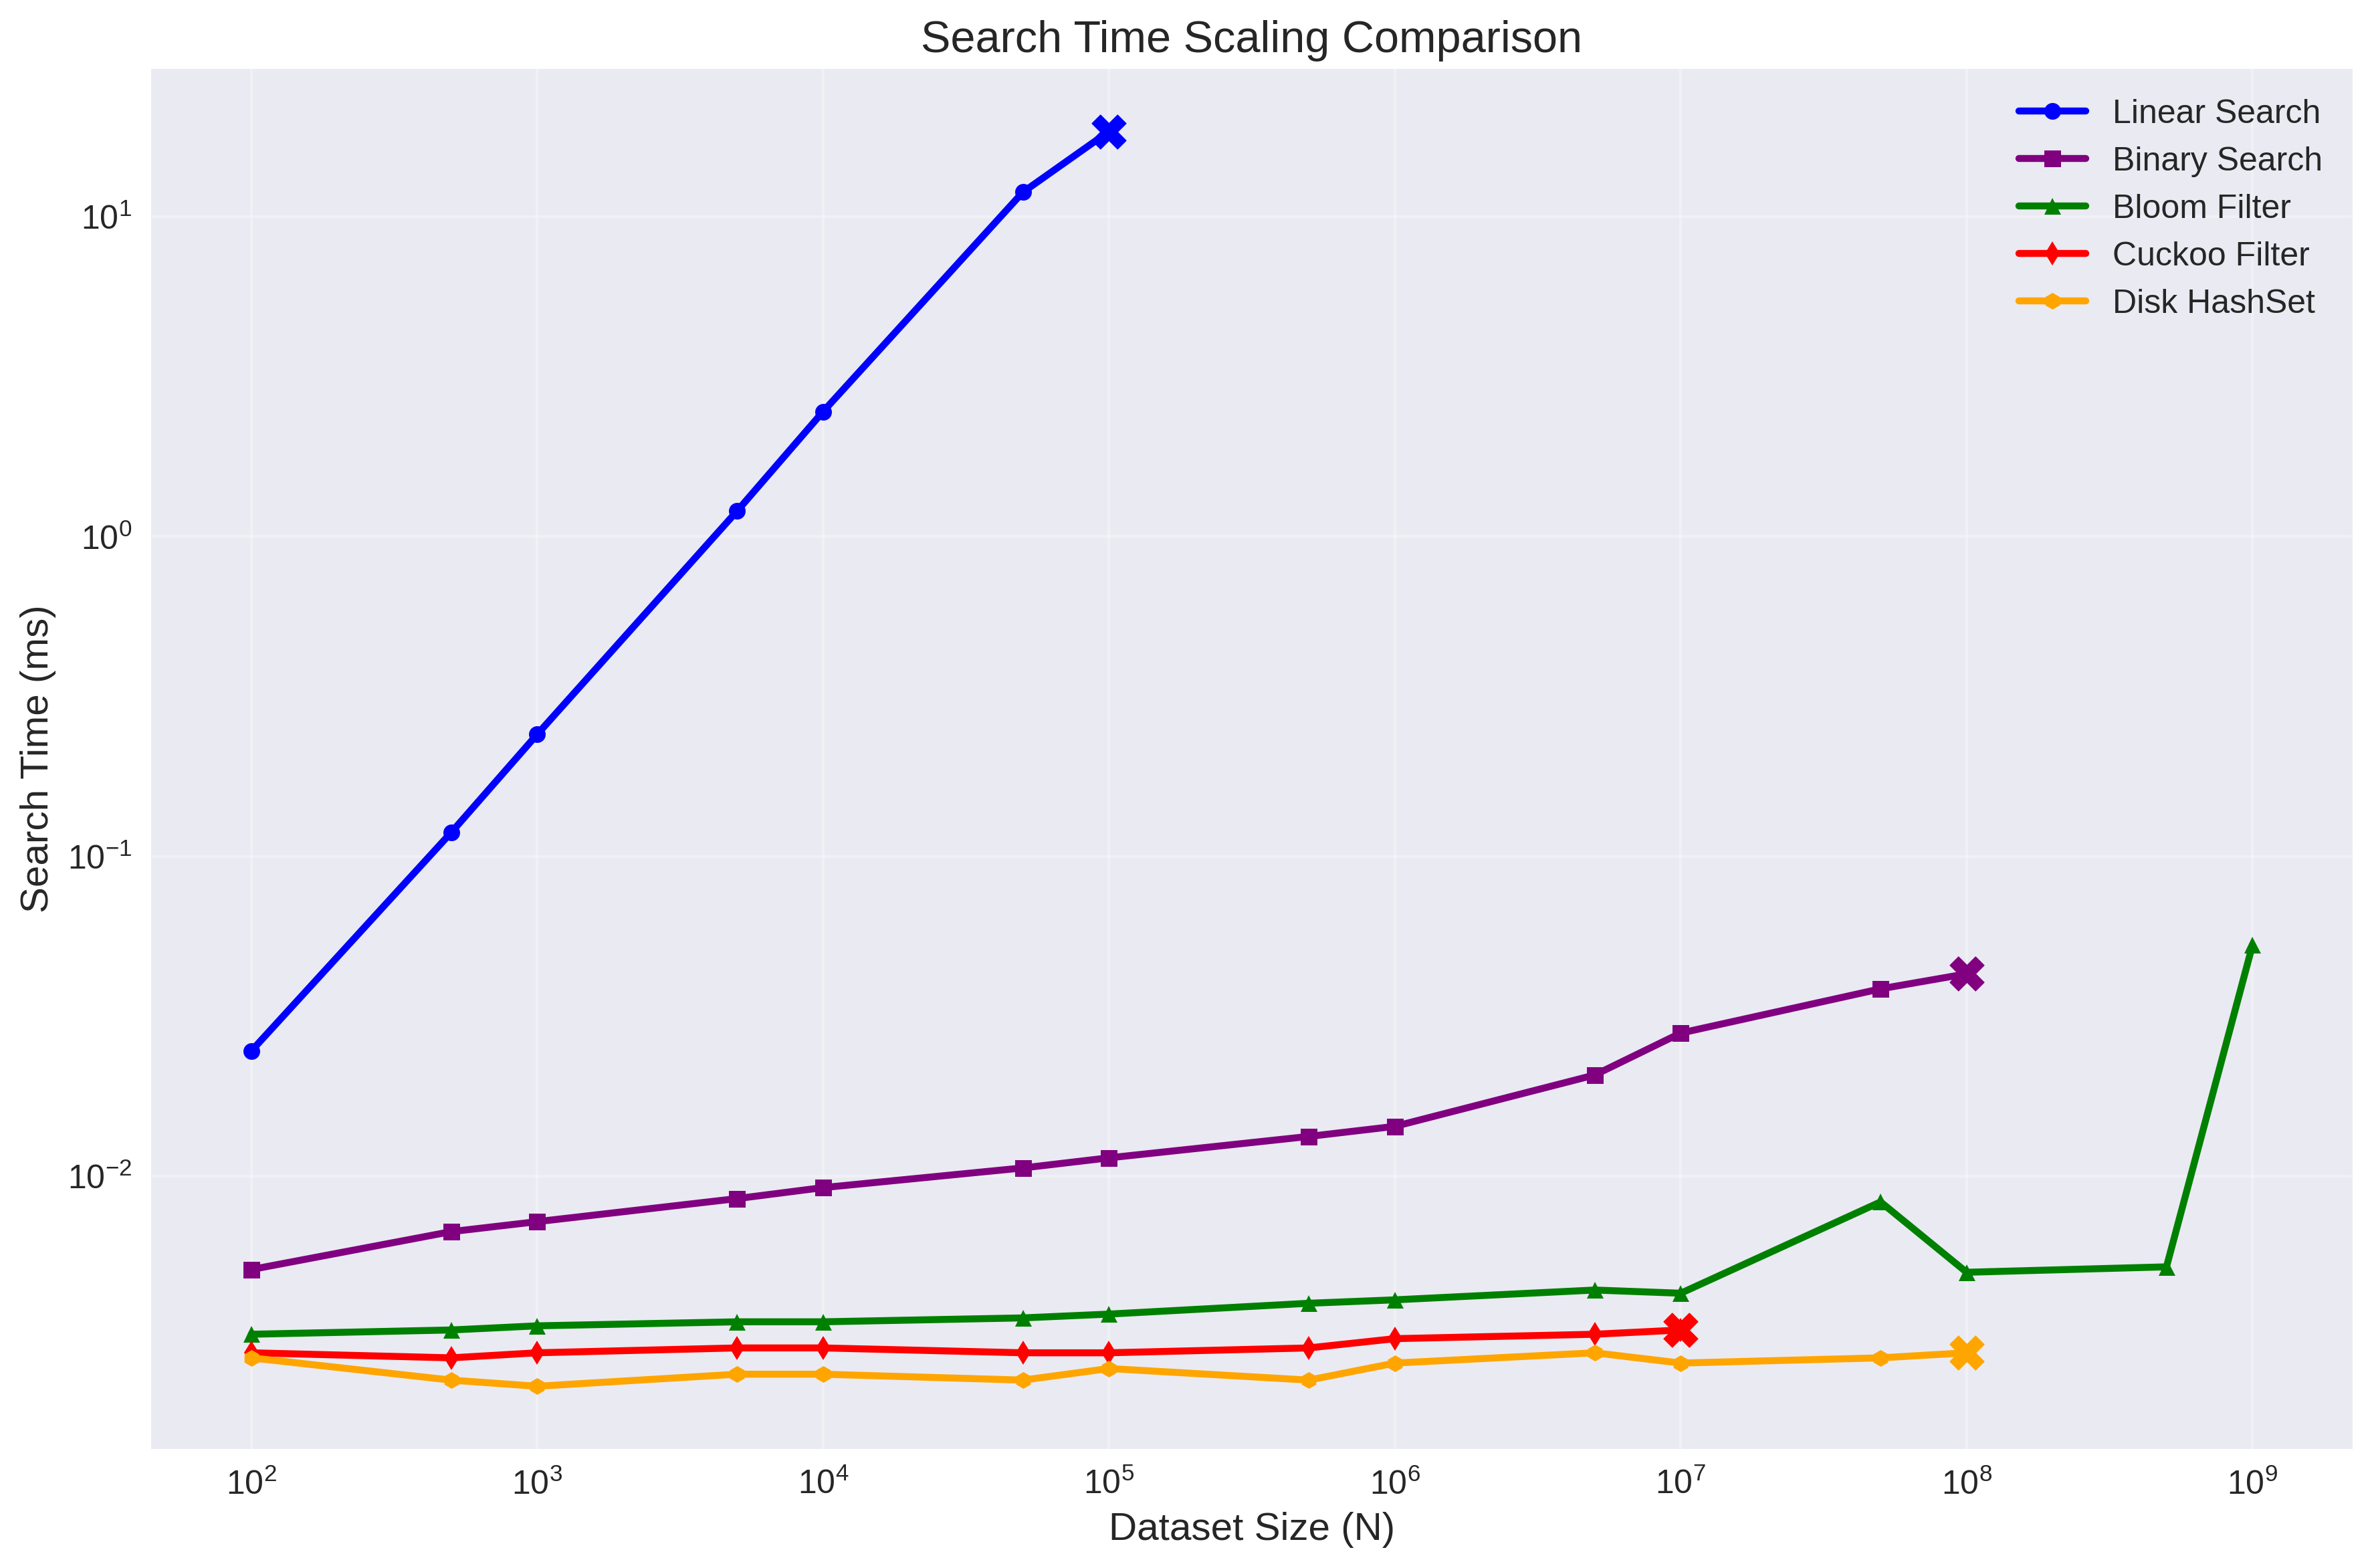
\includegraphics[width=0.95\linewidth]{search-time-scaling}
\caption{Search time scaling comparison showing all algorithms to their practical limits. X markers indicate where algorithms stop due to time constraints.}
\label{fig:search-time-scaling}
\end{figure}

\begin{figure}[h]
\centering
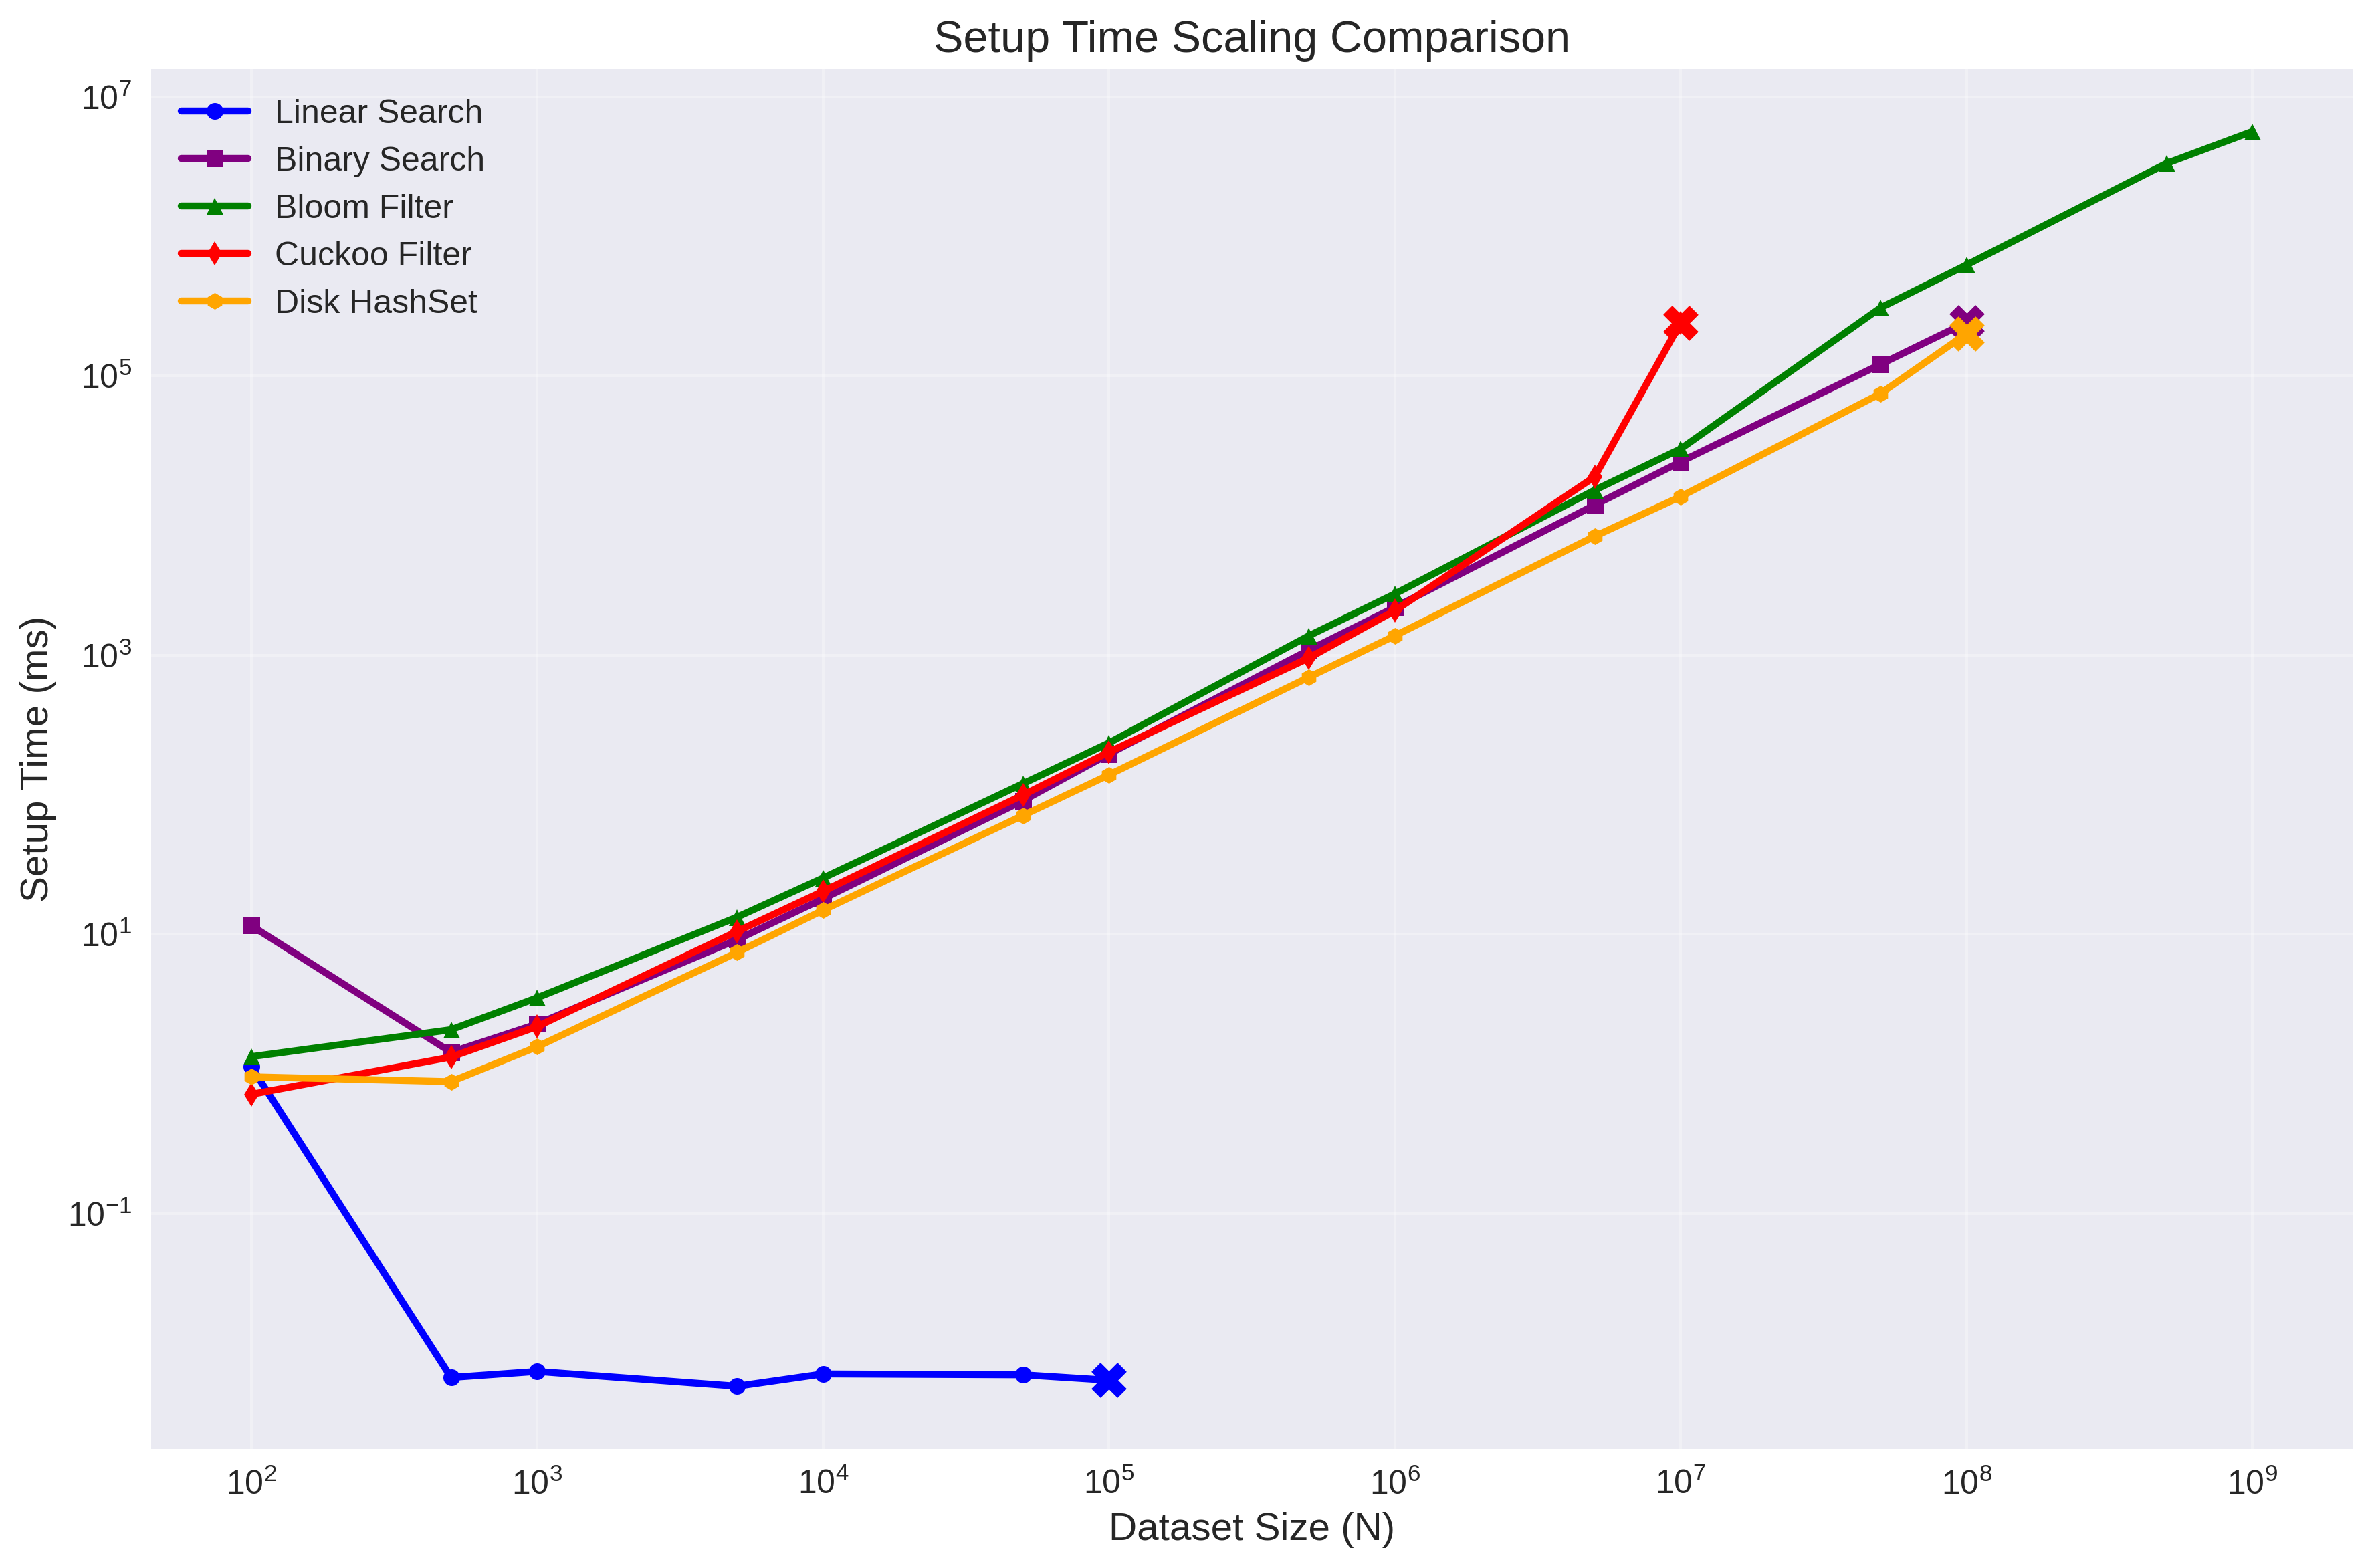
\includegraphics[width=0.95\linewidth]{setup-time-scaling}
\caption{Setup time scaling comparison across all algorithms. Shows the initialization overhead for each data structure.}
\label{fig:setup-time-scaling}
\end{figure}

\begin{figure}[h]
\centering
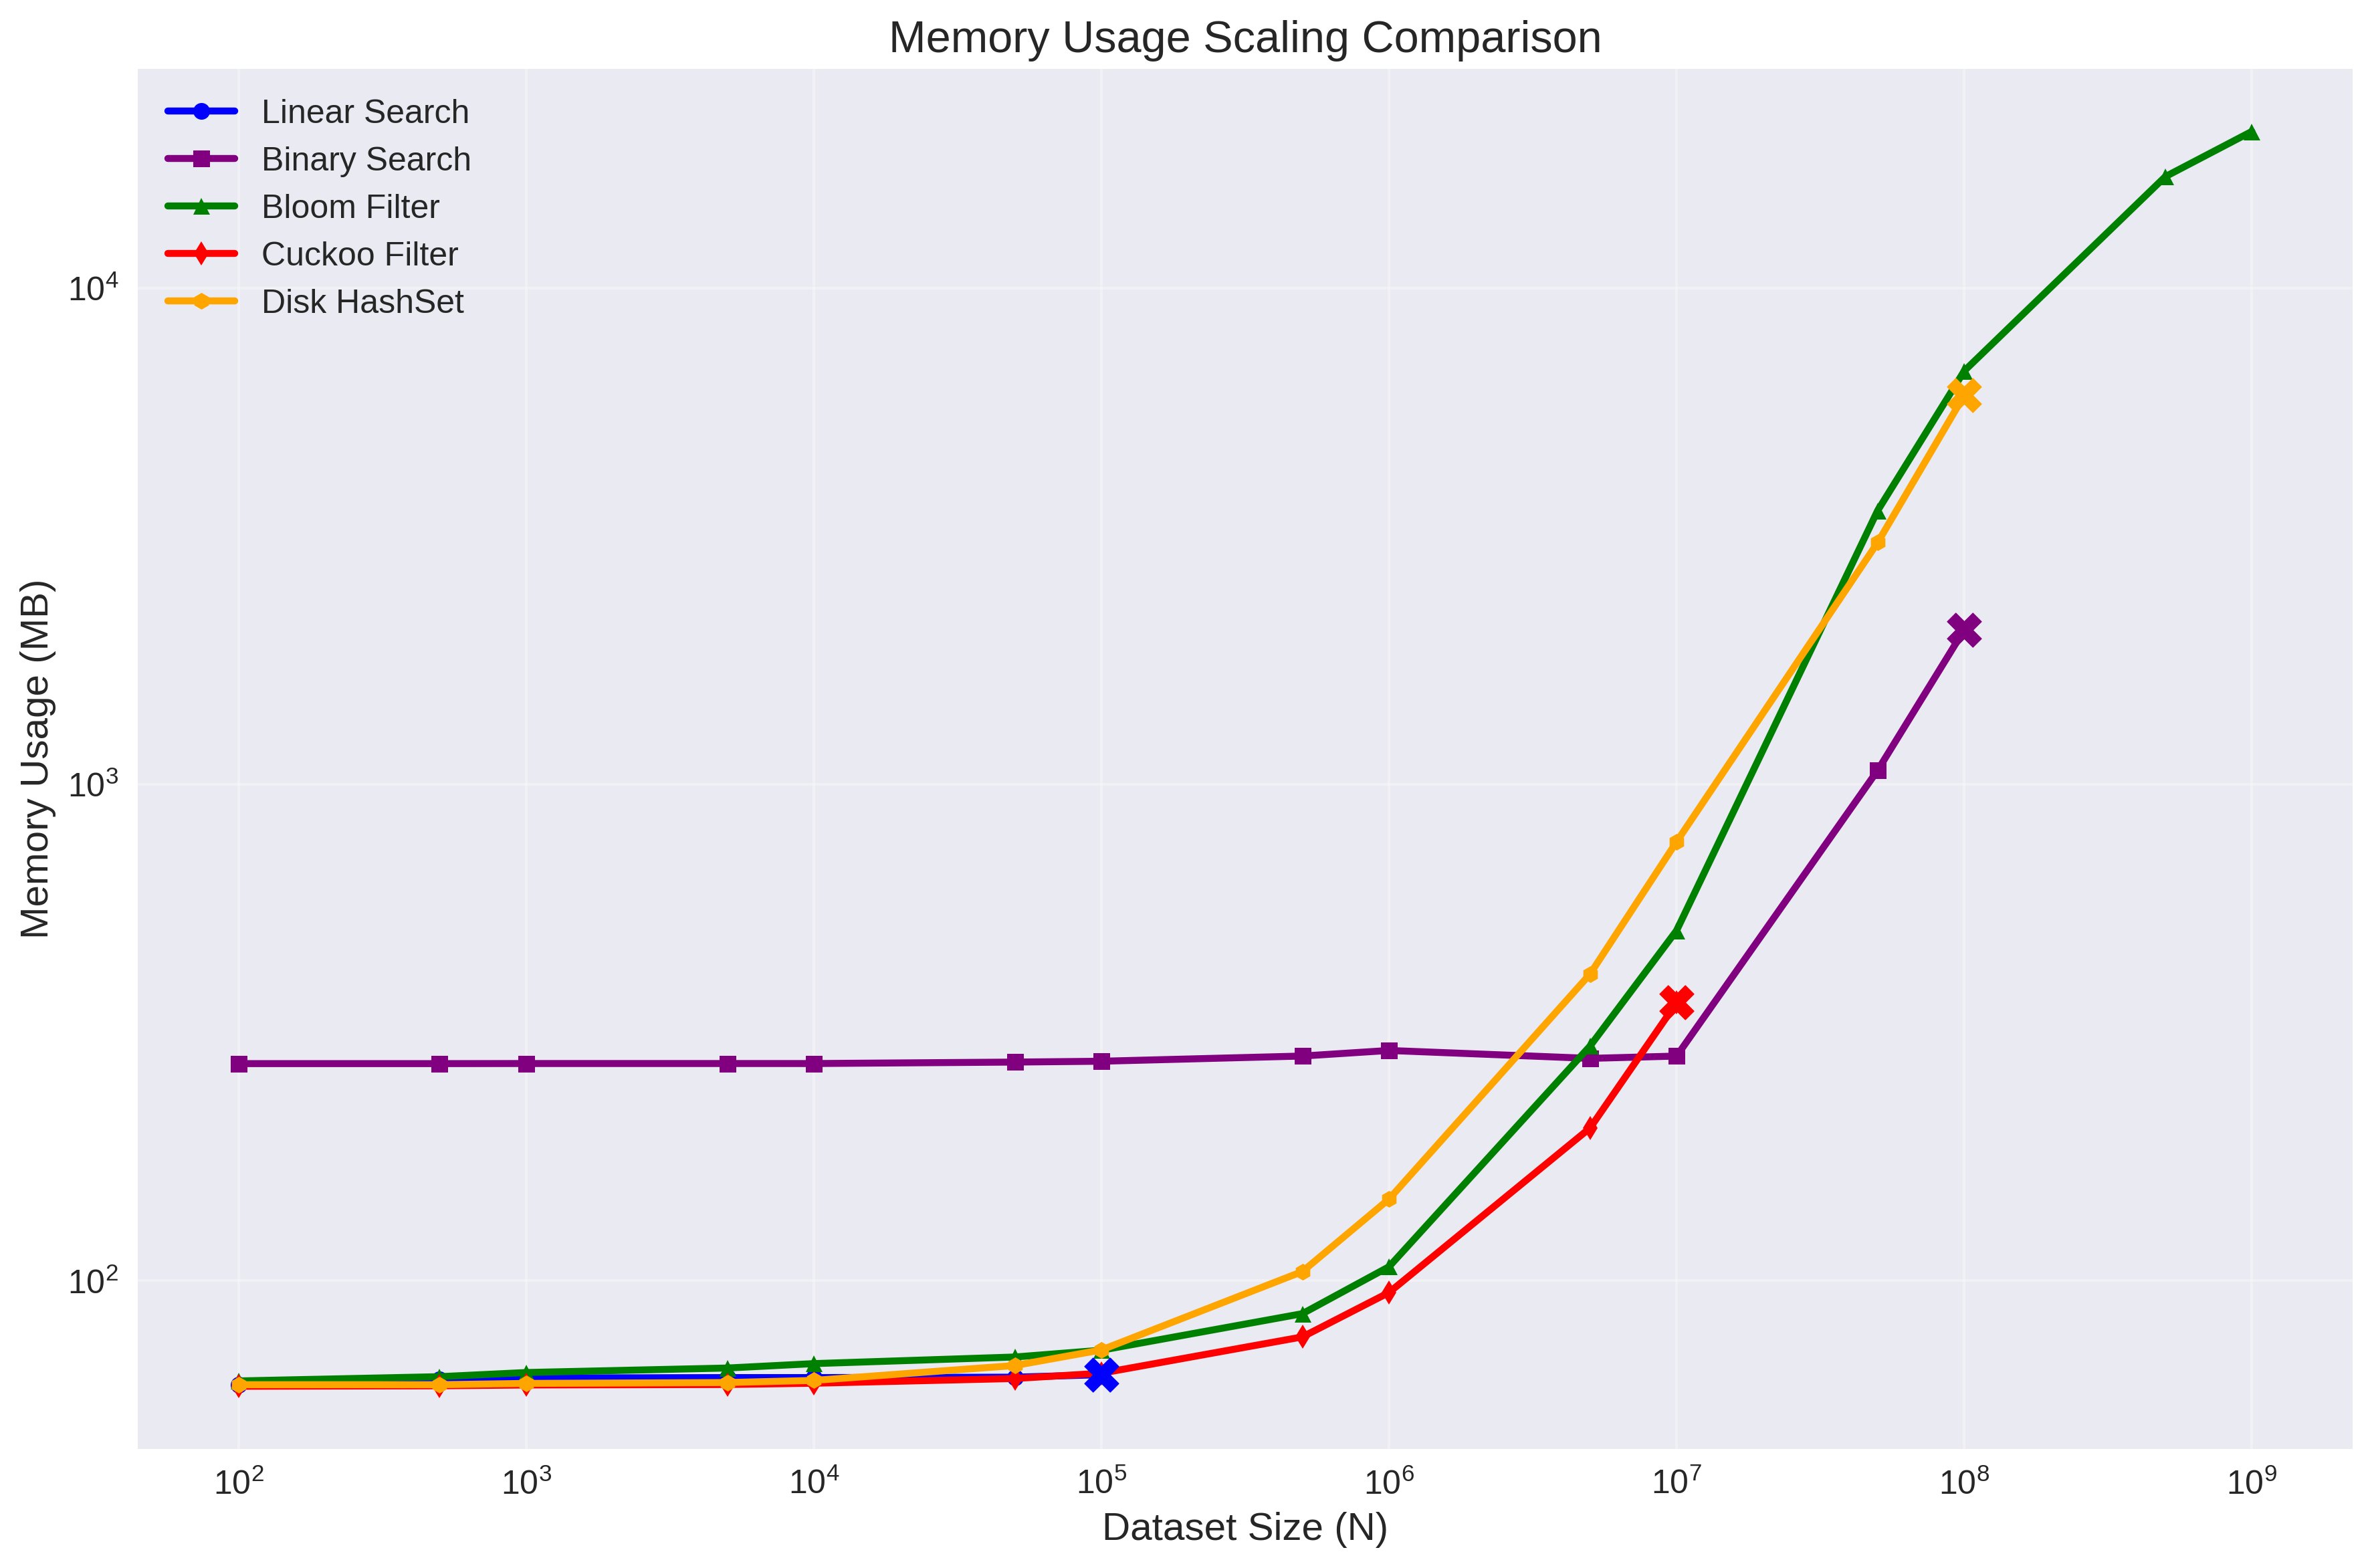
\includegraphics[width=0.95\linewidth]{memory-usage-scaling}
\caption{Memory usage scaling comparison. Linear search shows constant high memory usage due to implementation overhead.}
\label{fig:memory-usage-scaling}
\end{figure}

\begin{figure}[h]
\centering
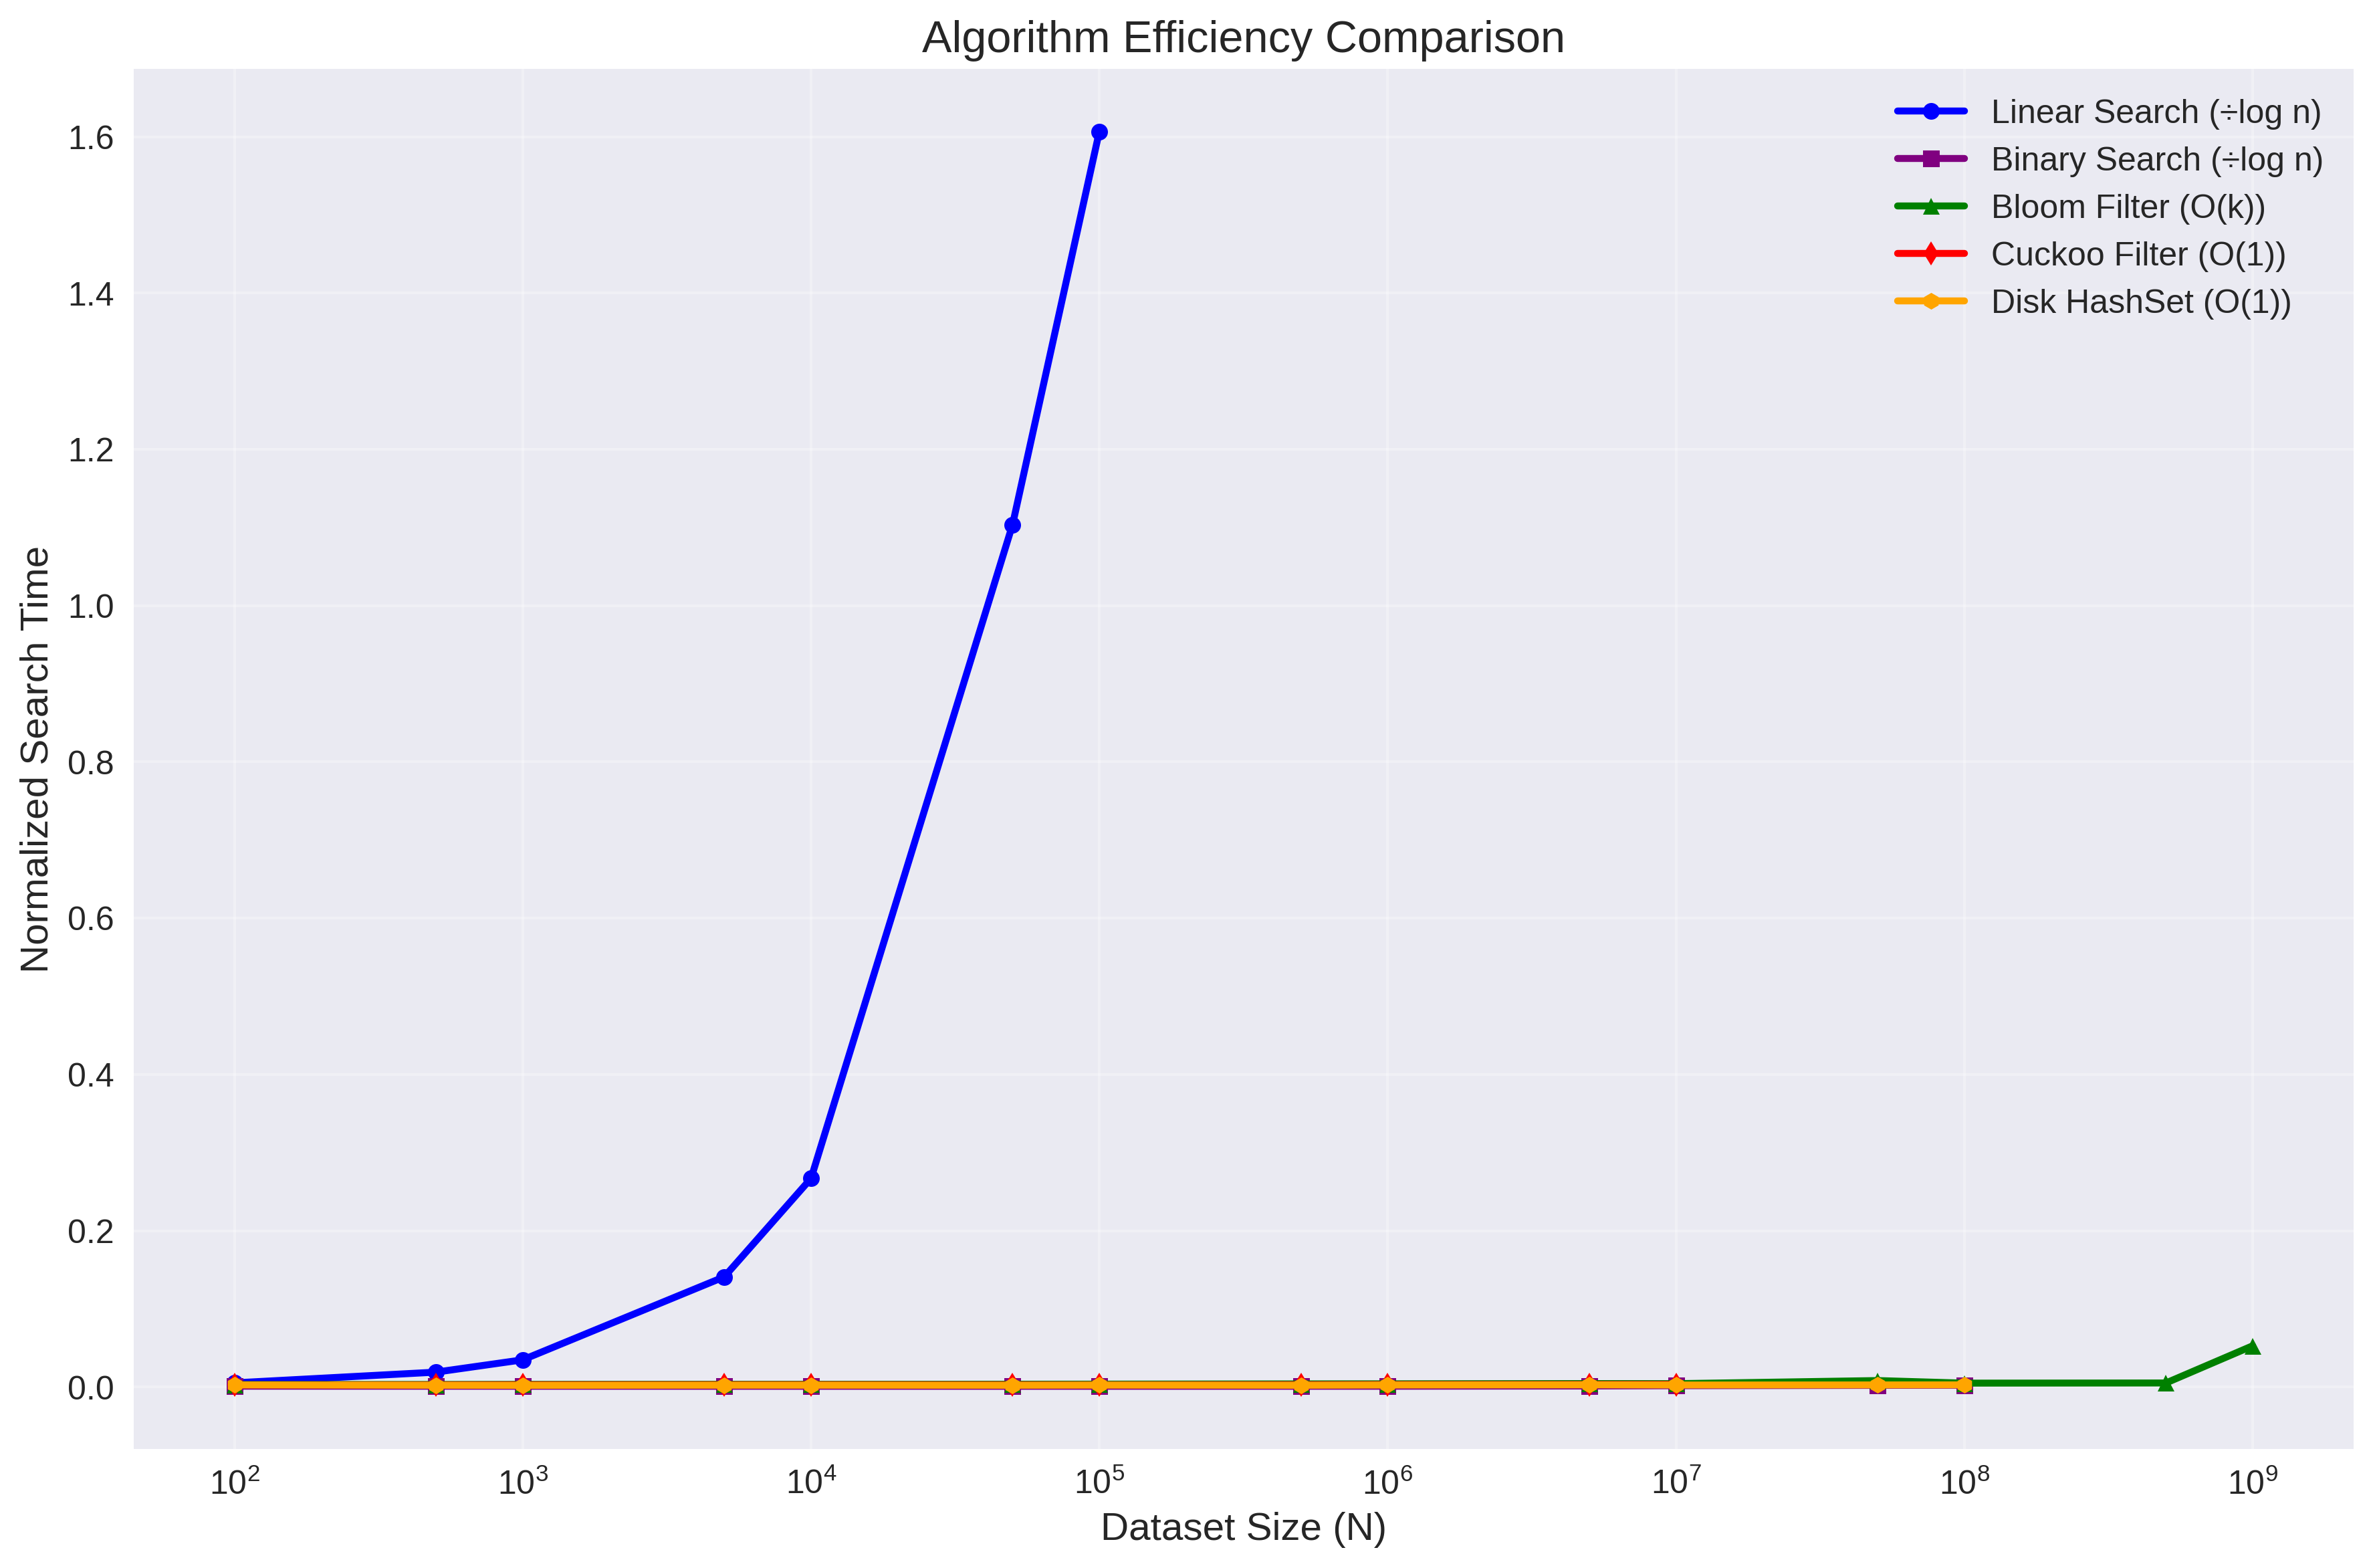
\includegraphics[width=0.95\linewidth]{efficiency-comparison}
\caption{Algorithm efficiency comparison with normalized metrics. O(1) algorithms show flat performance while O(log n) algorithms are normalized by log n.}
\label{fig:efficiency-comparison}
\end{figure}

\begin{figure}[h]
\centering
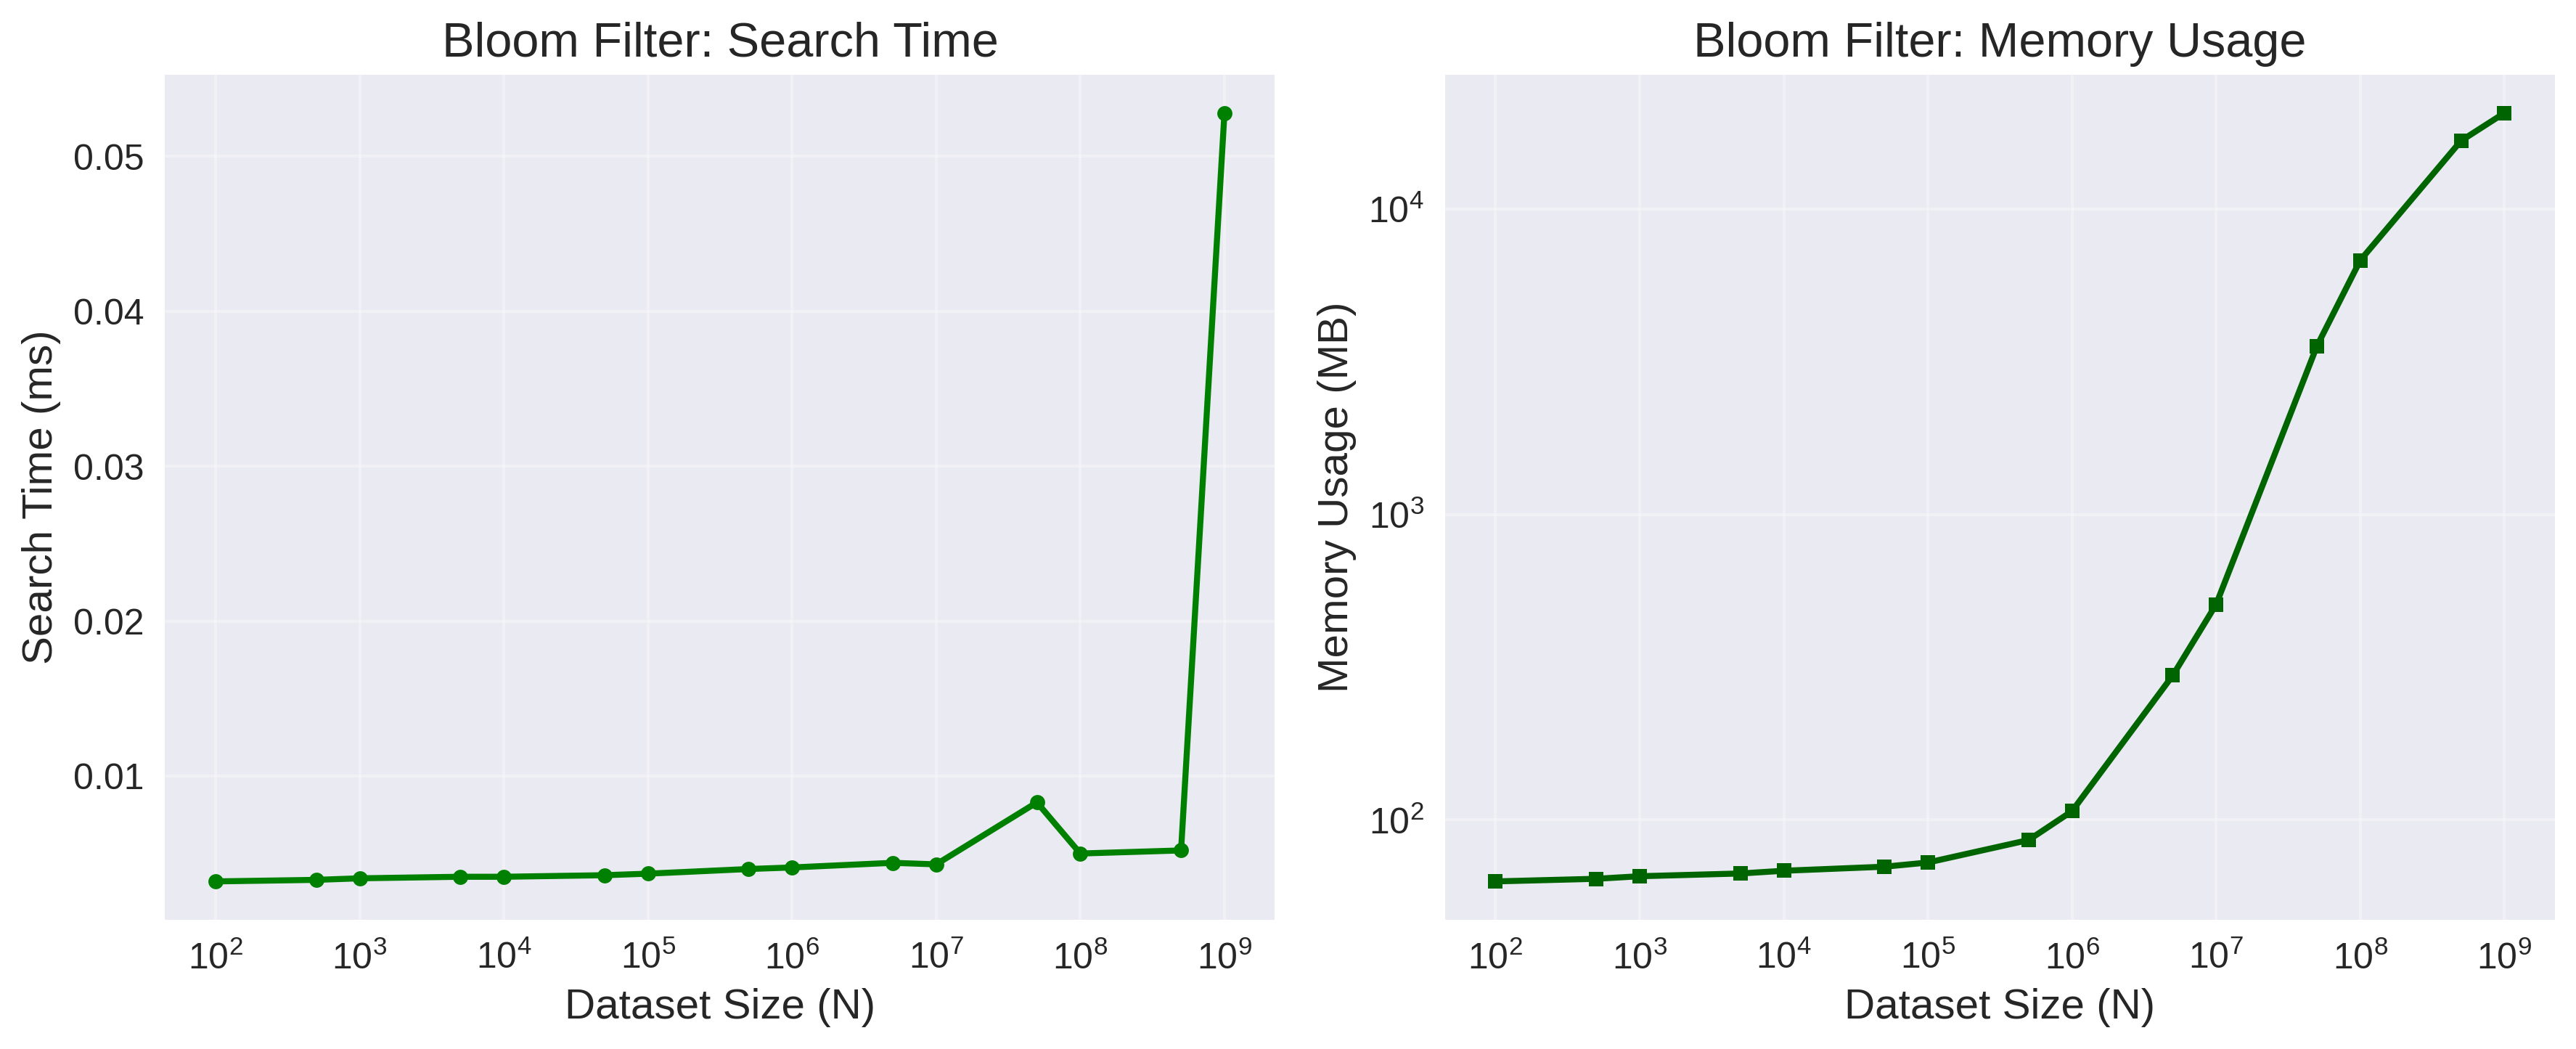
\includegraphics[width=0.95\linewidth]{bloom-filter-scaling}
\caption{Bloom filter scaling analysis: (left) search time remains consistent across all scales, (right) memory usage scales linearly with dataset size through memory-mapped storage.}
\label{fig:bloom-scaling}
\end{figure}

\section{Experimental Observations and Insights}
Based on my experimental validation (Tables~\ref{tab:linear-results}--\ref{tab:cuckoo-results} and summarized in Table~\ref{tab:algorithm-comparison}), I observed the following key characteristics:
\begin{itemize}
\item \textbf{Linear search:} Practical limit at 100K elements where search time reaches 18,500$\mu$s (Table~\ref{tab:linear-results}). The O(n) complexity makes it unsuitable for larger datasets.
\item \textbf{Binary search:} Tested successfully up to 100M elements with search times remaining under 43$\mu$s (Table~\ref{tab:binary-results}). The O(log n) scaling is evident in Figure~\ref{fig:search-time-scaling}.
\item \textbf{Disk HashSet:} Exceptional performance with consistent ~2.5$\mu$s search times across all tested scales (100 to 100M elements, Table~\ref{tab:disk-results}). The O(1) algorithmic complexity and memory-mapped architecture theoretically support billion-scale datasets, but such experiments were not conducted due to time constraints.
\item \textbf{Bloom filter:} Successfully scaled to 1 billion elements (Table~\ref{tab:bloom-results}). Search time remained under 6$\mu$s for most scales, with detailed scaling analysis shown in Figure~\ref{fig:bloom-scaling}.
\item \textbf{Cuckoo filter:} Consistent performance up to 10M elements with search times around 3$\mu$s (Table~\ref{tab:cuckoo-results}). The implementation used bucket size 4, target load factor 95\%, and maximum 500 kicks per insertion. While billion-scale experiments were not conducted due to time constraints (setup time for 1B elements is substantial), the O(1) algorithmic complexity and memory-mapped architecture theoretically support such scaling. At larger tested scales, insertion failures became significant: 50M elements experienced 2.5M insertion failures, while 100M elements had 5M insertion failures, demonstrating load factor management challenges.
\end{itemize}
\textbf{Key insight:} The disk-based implementation choice proved crucial for billion-scale experiments, allowing algorithms to handle datasets far exceeding available RAM through efficient memory mapping. Figure~\ref{fig:efficiency-comparison} illustrates the relative efficiency of each algorithm across different scales.

\textbf{Memory behavior observations:} The binary search memory measurements (Table~\ref{tab:binary-results}) show what appears to be nearly constant memory usage on a logarithmic scale, which reflects the RSS (Resident Set Size) memory measurement capturing data actively loaded into RAM from disk-based storage. As binary search accesses different portions of the sorted dataset through memory-mapped files, the OS loads relevant pages into memory, resulting in memory growth that follows the logarithmic access pattern of the algorithm. This behavior demonstrates that memory usage scales logarithmically with dataset size, corresponding to the portions of the dataset actively accessed during search operations rather than the entire dataset being held in memory simultaneously. Note that binary search is theoretically $\Theta(1)$ space complexity if we continuously flush back loaded pages to maintain constant memory usage, but since my implementation does not perform explicit page flushing, we observe this logarithmic memory growth pattern as accessed pages accumulate in RAM.

\textbf{Future work:} Due to time constraints, this study did not investigate: (1) billion-scale experiments for Disk HashSet and Cuckoo filter (both theoretically capable but requiring substantial setup time), and (2) the trade-offs between time complexity, space complexity, and false positive rates for the probabilistic structures. Such analysis would provide valuable insights into optimal parameter selection for different application requirements and complete billion-scale validation across all O(1) algorithms.

\section{Acknowledgments}
This report was prepared with assistance from Generative AI, specifically Claude Sonnet 4, for data analysis, plot generation, and document formatting. The experimental design, implementation, and interpretation of results remain the author's original work.

\section{Code and Reproducibility}
All experiments use deterministic seeds for reproducibility. Memory-mapped storage enables billion-scale experiments on standard hardware.

\section{Conclusion}
This study provides comprehensive analysis of five membership testing algorithms for billion-scale username datasets, with a focus on disk-based implementations for practical scalability.

\textbf{Key findings:} Disk-based hash tables demonstrate exceptional performance with consistent ~2.5$\mu$s search times across all tested scales (100 to 100M elements), proving the effectiveness of memory-mapped storage for large-scale applications. Bloom filters were experimentally validated up to 1 billion elements while maintaining sub-microsecond search times for most scales. Both disk-based hash tables and Cuckoo filters are theoretically capable of billion-scale performance, but experimental validation was limited by setup time constraints. Linear search becomes impractical beyond 100K elements (18,500$\mu$s search time), while binary search remains efficient up to 100M elements.

\textbf{Implementation contributions:} The disk-based approach using memory-mapped files enables processing of datasets exceeding available RAM (memory scaling shown in Figure~\ref{fig:memory-usage-scaling}). The implementation uses MurmurHash3~\cite{mmh3docs} for consistent hashing, fixed 32-byte slots for predictable performance, and Kirsch-Mitzenmacher optimization~\cite{kirsch2008} for Bloom filters.

\textbf{Practical implications:} For exact membership testing at scale, disk-based hash tables provide optimal performance. For applications tolerating false positives, Bloom filters offer excellent scalability.

Complete implementation available~\cite{loginchecker}.




%%
%% The next two lines define the bibliography style to be used, and
%% the bibliography file.
\bibliographystyle{ACM-Reference-Format}
\begin{thebibliography}{9}
\bibitem{bloom1970}
B. H. Bloom. Space/time trade-offs in hash coding with allowable errors. Communications of the ACM, 13(7):422–426, 1970.

\bibitem{kirsch2008}
A. Kirsch and M. Mitzenmacher. Less hashing, same performance: Building a better Bloom filter. Random Structures \& Algorithms, 33(2):187-218, 2008.

\bibitem{fan2014}
B. Fan, D. Andersen, M. Kaminsky, and M. Mitzenmacher. Cuckoo Filter: Practically Better Than Bloom. CoNEXT 2014.

\bibitem{mmh3docs}
Hajime Senuma. mmh3 documentation. \url{https://mmh3.readthedocs.io/en/latest/}, 2025.

\bibitem{mimesis}
Isaak Uchakaev. Mimesis: Fake Data Generator. \url{https://mimesis.name/master/}, 2025.

\bibitem{loginchecker}
Fahd Seddik. LoginChecker: Membership Testing Algorithms Implementation. \url{https://github.com/FahdSeddik/LoginChecker}, 2025.

\bibitem{bloomhash}
Stack Overflow. Which hash functions to use in a bloom filter. \url{https://stackoverflow.com/questions/11954086/which-hash-functions-to-use-in-a-bloom-filter}, 2012.

\bibitem{fnvgist}
ruby0x1. FNV1a hash implementation. \url{https://gist.github.com/ruby0x1/81308642d0325fd386237cfa3b44785c#file-hash_fnv1a-h-L25}, GitHub Gist.

\bibitem{fnvofficial}
Landon Curt Noll. FNV Hash - Fowler-Noll-Vo hash function. \url{http://isthe.com/chongo/tech/comp/fnv/#FNV-1a}, 2024.

\bibitem{stringhash}
Stack Overflow. Best string hashing function for short filenames. \url{https://stackoverflow.com/questions/11413860/best-string-hashing-function-for-short-filenames}, 2012.

\end{thebibliography}

\appendix
\section{Implementation Details}
\subsection{Memory Management}
All data structures use memory-mapped files for efficient handling of large datasets:
\begin{itemize}
\item Automatic virtual memory management by the OS
\item Minimal RAM usage regardless of dataset size
\item Persistent storage with crash recovery
\end{itemize}

\subsection{Hash Function Selection}
MurmurHash3~\cite{mmh3docs} was chosen for all implementations due to:
\begin{itemize}
\item Excellent distribution properties for string keys
\item High performance (faster than cryptographic hashes)
\item Widely tested and validated in production systems
\item Consistent 64-bit output across platforms
\end{itemize}

\end{document}
